\chapter{ゴルフスイングのバイオメカニズム}
\section{バイオメカニクス}
%
バイオメカニクス(biomechanics)とは,生体に力が作用して起こる現象を取り扱う,力学の一分野であり,日本語では生体力学,あるいは生体機械工学とも呼ばれる.
バイオメカニクスでは,ヒトをはじめとする全生物を対象とし,対象の生物の器官系,器官,組織,細胞,遺伝子といった,各レベルまで扱う.
バイオメカニクスの歴史として,14世紀から16世紀に急速にヒトの内部の仕組みを知りたいという願望が増大し,その中でも,レオナルド・ダ・ビンチが人体解剖図を精密がしたことが有名である.

現在のバイオメカニクスは,バイオメカニクスと関連した学問や分野が発展し,解剖学,生理学,医用工学,人間工学,スポーツ工学といった分野がよく関連されている.
%
\section{人体構造}
図\ref{基本的立位姿勢}は基本的立位姿勢を示す.
\begin{figure}
    \begin{center}
        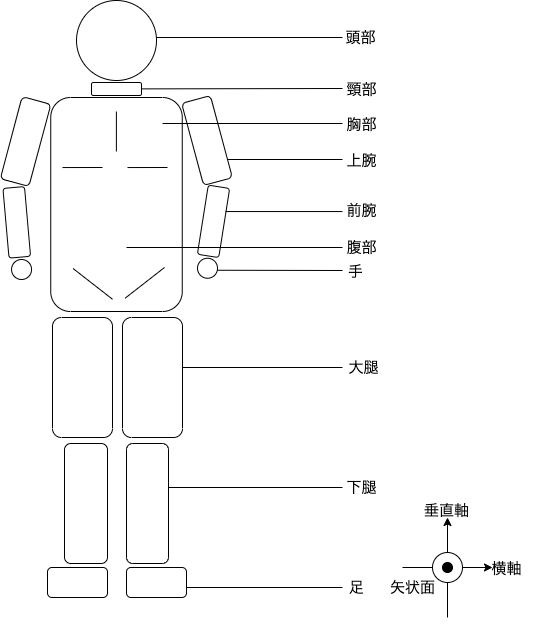
\includegraphics[width = 5cm]{./images/human_body.png}
        \caption{基本的立位姿勢}
        \label{基本的立位姿勢}
    \end{center}
\end{figure}
ヒトには,いくつかの部位のグループで呼ばれることがある.
一般に体幹と呼ばれるグループがあるが,
広い幅の意味を持つ体幹とは図\ref{基本的立位姿勢}より,頭部,頸部,胸部,腹部のグループであり,その中でも胸部,腹部のみでも体幹と呼ばれることがある.
上腕,前腕,手の三部位を総称し上肢と呼び,大腿,下腿,足の三部位を総称し下肢と呼ぶ.
また,上肢,下肢を総称し体肢,四肢と呼ばれることがある.
% 本研究もこの名称に従い,部位の名称を扱う.

次に,運動の基準とする軸について説明する.
図\ref{基本的立位姿勢}より,床と頭部を結ぶ軸を垂直軸,床と左右に並行の軸を横軸,背面から前方方向への軸を矢状軸と呼ぶ.


% \section{関節}
% 本節ではヒトの関節名称を示す.
% \begin{figure}
%     \begin{center}
%         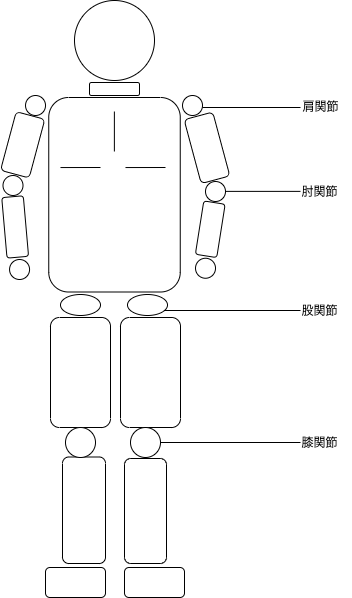
\includegraphics[width = 5cm]{./images/joint.png}
%         \caption{関節構造}
%         \label{関節構造}
%     \end{center}
% \end{figure}
% 図\ref{関節構造}の,

\section{人体の運動表現}
ヒトが運動する際に,その時の運動の表現は世界共通の表現がある.
本節では,日本整形外科学会の規則に則り,ヒトの運動表現について説明を行う.

ヒトには,屈曲/伸展,外転/内転,外旋/内旋の三種類の基本動作がある.
屈曲/伸展とは,横軸に並行な運動である.
一般に,頭部,胸部が前方に倒れる方向を屈曲,反対の動きを伸展と呼ぶ.
外転/内転とは,矢状軸に並行な運動である.
一般に,上肢を床と並行,矢状軸と直角になる運動を外転,反対の動きを内転と呼ぶ.
また,頸部,胸部,腰部は定義に則した運動に一致しないことから,側屈と呼ばれることがある.
外旋/内旋とは,垂直軸に並行な運動である.
一般に,前腕を床と並行かつ上腕と直角にした状態で,上体の方向に回転する運動を内旋,上体から離れるような回転を外旋と呼ぶ.
また,頸部,胸部,腰部は定義則した運動に一致しないことから,回旋や捻転と呼ばれることがある.

\section{ゴルフ}
%
現在,日本のゴルフはかなり盛んであり,プロゴルファーの松山や渋野が海外で活躍するのをきっかけに,全世代的に見ても流行の兆しがある.
特に,日本のゴルフ用品の市場規模は,世界二位の2000億円であり,ますます期待されるのスポーツである.

ゴルフの初心者等は,上達のためにスクールに通いインストラクターをつけ,最新の器具や設備,解析機器を使用して練習に励む動向がある.
特に現代の技術では,
ハイスピードカメラや高性能カメラを使用したモーションキャプチャを用いたゴルフスイング解析,
トラックマンを使用したゴルフボールの弾道測定,
また,動画技術も向上したため様々な流儀のスイング解説がある.

ゴルフとは,最小打数でボールをカップに入れること競うスポーツである.
ゴルフをプレーするにあたり,フィールドが用意されているが,ゴルフでは打ち初めからカップに入れるまでにプレーを行うフィールドをホールと呼ぶ.
各ホールには規定打数が決められており,3打数(パー3)が4ホール,4打数(パー4)が10ホール,5打数(パー5)が4ホールの計18ホール(1ラウンド)があり,1ラウンドを規定打数通りにプレーすると72打数で終了することとなる.

各ホールには,5つのエリアが定義されている.
5つのエリアとは,
プレイヤーが必ず打ち始めを行うティーイングエリア,
フェアウェイ,ラフ,その他の自然物を含めたジェネラルエリア,
プレイヤーの能力をテストするために特別に設置されたバンカーエリア,
ボールを地面で転がしカップに入れること目的としたパッティンググリーン,
そして,主にプレーを続行することが不能となりペナルティーが課せられるペナルティーエリアがある.

ゴルフの競技性として,規定打数より少ない打数でカップに入れられたプレイヤーが勝利となるため,プレイヤーは,ティーイングエリアからスタートしパッティンググリーンのカップへ効率良くいれることが必要である.
故に,バンカーエリアやペナルティーエリアをさけ,可能な限りジェネラルエリア,特にフェアウェイ上でプレイされることが望ましい.

\section{ゴルフボールの弾道}
ゴルフの基本として,真っ直ぐかつ遠くに飛ばすことが理想であるが,一般ゴルファーには右に曲がってしまうスライス弾道や,左に曲がるフック弾道となってしまうことがある.
スライス弾道のメカニズムは,クラブフェースがボールに対し右向きでヒットすることにより,ボールの回転が右回転するためである.
クラブフェースが右向きでボールにヒットすることを,オープンフェースと呼ばれるが,オープンフェースの主な原因は,クラブの軌道がインサイドアウトになってしまうことである.
フック弾道のメカニズムは,クラブフェースがボールに対し左向きでヒットすることにより,ボールの回転が左向きになるためである.
クラブフェースが左向きでボールにヒットすることを,クローズフェースと呼ばれるが,クローズフェースの主な原因は,クラブの軌道がアウトサイドインになってしまうことである.
すなわち,ゴルフボールを真っ直ぐに飛ばすためには,クラブフェースがボールに対し並行(スクエアフェース)でヒットすることが重要であり,これを実現するためには,クラブがインサイドインの軌道を描くことが需要である.

一般ゴルファーや初心者ゴルファーは,スライス弾道になってしまうことがよくあるが,その原因としてヘッドアップ動作や身体が開く動作が原因として上がる.
次節にて,ヘッドアップ動作,身体が開く動作について説明する.

\section{ヘッドアップ動作と身体が開く動作}
前節にて,一般ゴルファーや初心者ゴルファーにはヘッドアップ動作や身体が開く動作がよく起こると述べた.

\begin{figure}
    \begin{center}
        \begin{tabular}{c}
            \begin{minipage}{0.5\hsize}
                \begin{center}
                    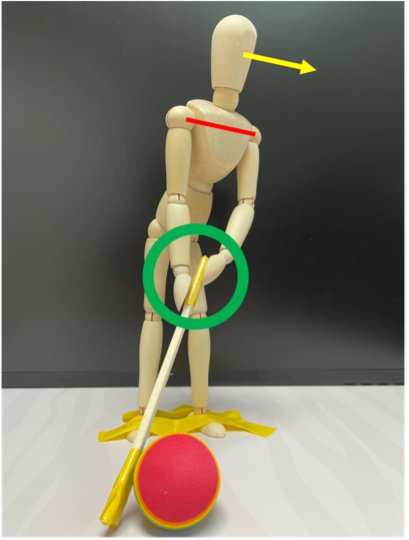
\includegraphics{./images/headup.png}
                    \caption{ヘッドアップ動作}
                    \label{headup}
                \end{center}
            \end{minipage}

            \begin{minipage}{0.5\hsize}
                \begin{center}
                    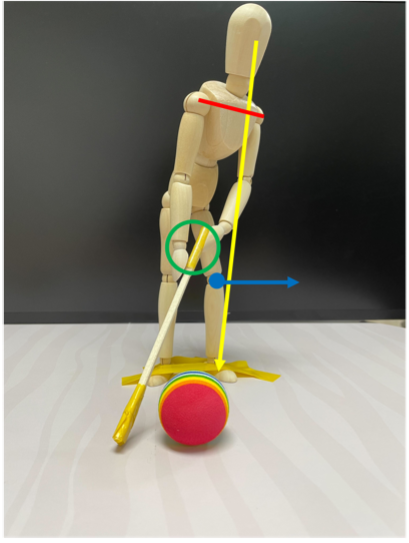
\includegraphics{./images/opening.png}
                    \caption{身体が開く動作}
                    \label{opening}
                \end{center}
            \end{minipage}
        \end{tabular}
    \end{center}
\end{figure}

ヘッドアップ動作とは,\ref{headup}の黄色線のように目線がインパクトする前に打球方向へ向いてしまう動作である.
また,アドレス時の前傾姿勢をインパクト時まで保てずに頭部が起き上がる動作もヘッドアップに分類される.
この動作により,図1の赤線のようにインパクト前に上半身が起き上がり図1の緑円ように腕が振り遅れるため,
ゴルフクラブのフェースの開きが誘起され,結果としてスライス弾道が起こる.

身体の開きの動作とは,\ref{opening}の赤線や青線のようにヒトの正面胸部や前足軸の膝がインパクトより前に打球方向へ向いてしまう動作である.
この動作もヘッドアップ動作同様で,図2の緑円のように上体より腕が振り遅れてしまうため,ゴルフクラブフェースの開きが誘起される.

ヘッドアップ動作やインパクト前の身体の開きは,スイングを撮影した動画を見ただけでは初心者やアベレージゴルファーにとっては,特定するのは非常に困難であることが知られている.
また,その動作がどの部位にどのタイミングで起こっていることを特定することは非常に困難である.
そこで,本研究では特にスライス弾道の原因となるヘッドアップ動作とインパクト前の身体の開き動作に焦点をあて,頭部と身体の開き関係する関節部に注目してスイングの解析を行う.
本研究は,スライス弾道の大きな原因と言われるヘッドアップ動作,身体の開きの動作より,頭部と身体の開き関係する関節部に注目して解析を行う.